\documentclass{article}[H]
\usepackage[utf8]{inputenc}
\usepackage{geometry}
\geometry{
 a4paper,
 left=25.4mm,
 top=25.4mm,
 }
\usepackage[spanish]{babel}
\usepackage{natbib}
\usepackage{graphicx} 
\graphicspath{{../fig/}}  
\usepackage{wrapfig}
\usepackage{subcaption}
\usepackage{caption}
\usepackage{float} 
%\usepackage{todonotes}
%\newcommand{\toask}[2][]{\todo[#1,color=green!60]{#2}}
%\newcommand{\test}[2][]{\todo[#1,color=red!60]{#2}}
%\newcommand{\done}[2][]{\todo[#1,color=blue!60]{#2}}
\usepackage{hyperref}
\hypersetup{colorlinks=false}


\title{\textbf{Documento de especificación de las pruebas de EEM} \\
\large Evaluación de estrategias de manejo pesquero (EEM) para el stock de anchoveta del norte de Chile en el contexto del enfoque precautorio de la Ley General de Pesca y Acuicultura.}

\author{}

\date{}

\begin{document}
 
\maketitle

\section{Introducción}

% !TeX root = ../Doc_especific_mse_anchovy.tex


En febrero del año 2023, se publicó en el Diario Oficial de Chile la Ley 20.657, \textit{Ley General de Pesca y Acuicultura} (LGPA), que cambio el paradigma predominante de manejo pesquero en Chile, debido a que el estado de explotación de las principales pesquerías nacionales se encontraba en su mayoría sobreexplotadas e incluso algunas en estado de colapso, siendo urgente poner a la conservación y el uso sostenible de los recursos como uno de los ejes rectores de la regulación de la actividad pesquera. Entre estos cambios, fue la adopción del enfoque de precautorio para la pesca \citep{FAO1997}, el enfoque ecosistémico para la pesca \citep{FAO2003} y el \textit{Rendimiento Máximo Sostenible} (RMS, \cite{maunder20089th}) basados en objetivos de manejo pesquero \citep{reyes2017problemas}. Con esta legislación, además se establecieron los comités científicos técnicos y de manejo pesquero y se confirió mayor peso al asesoramiento científico en el proceso de toma de decisiones para establecer los niveles de captura \citep{leal2011informe}.
\newline

La LGPA introdujo el requisito de \textit{Planes de Manejo Pesqueros} obligatorios (PMP) en su Título II, Párrafo 3$^\circ$ LGPA). Estos instrumentos de manejo vinculante deben especificar los objetivos, las metas y el período para reconstruir o mantener las poblaciones de peces al nivel del RMS junto con las estrategias para alcanzar los objetivos y metas establecidos. El PMP para la anchoveta y sardina española de las Regiones de Arica y Parinacota, Tarapacá hasta la Región de Antofagasta fue aprobado mediante Resolución Exenta N$^\circ$ 1197 del 9 de abril del 2018. El PMP declara una serie de objetivos operacionales asociados a estándares de manejo (indicador y punto de referencia) con los cuales se debe medir el progreso de la pesquería como consecuencia de la aplicación de medidas y/o acciones de manejo. Estos objetivos fueron sistematizados en cuatro dimensiones: biológica, ecológica, económica y social.
\newline

Para el caso de la dimensión biológica, el PMP declara llevar y mantener el stock de anchoveta a un nivel que permita asegurar la sustentabilidad biológica del recurso. Para tal efecto, el objetivo N$^\circ$1.1 es llevar y mantener el recurso al RMS, y la medida de manejo asociada a este objetivo es establecer una \textit{Captura Biológicamente Aceptable} (CBA) basada en los \textit{Puntos Biológicos de Referencia} (PBR, Res. Ex. N$^\circ$ 291 del año 2015). Para el caso del stock de anchoveta del norte de Chile se establecieron proxies al RMS \citep{Paya2014}, los cuales fueron ratificados por el \textit{Comité Científico Técnico de Pequeños Pelágicos} (CCT-PP). Para la \textit{Biomasa Desovante al RMS} (BDRMS) se estableció un valor igual al 50\% de la biomasa desovante virginal (BD0) y para la mortalidad por pesca al RMS (FRMS) se estableció aquella mortalidad por pesca que en el largo plazo produce el 55\% de la biomasa desovante por recluta (F55\%BDPR). La regla de control para este objetivo es aplicar una mortalidad por pesca constante al nivel del RMS.
\newline

La \textit{Evaluación de Estrategia de Manejo} (EEM) es el uso de la simulación para evaluar el desempeño de una combinación de métodos de evaluación de poblaciones y reglas de control de captura (estrategias de ordenación) ante la incertidumbre de objetivos pre-acordados \todo{No lo encuentro}(Smith et al. 1999). El enfoque de EEM implica el desarrollo de un marco que considere el sistema de manejo pesquero en su totalidad, incluida la dinámica poblacional de los peces, el esquema de recopilación de datos, el método de evaluación de poblaciones utilizado al proporcionar asesoramiento para el manejo pesquero y cualquier regla de control de captura. El enfoque EEM es totalmente consistente con el enfoque precautorio de la FAO para la ordenación pesquera \citep{tsukamoto2008refocusing}. Sin embargo, aún no se ha evaluado formalmente el desempeño de las estrategias de manejo candidatas para la anchoveta del sur de Perú y el norte de Chile. En este escenario, los objetivos de una correcta EEM deben estar consensuados entre el equipo de científicos (Instituto de Fomento Pesquero, IFOP), el sector pesquero (Comité de manejo) y el sector administrativo (Subsecretaria de Pesca y Acuicultura, SUBPESCA).



\subsection{Especie estudiada}

% !TeX root = ../Doc_especific_mse_anchovy.tex

\begin{figure}[h]
    \centering
    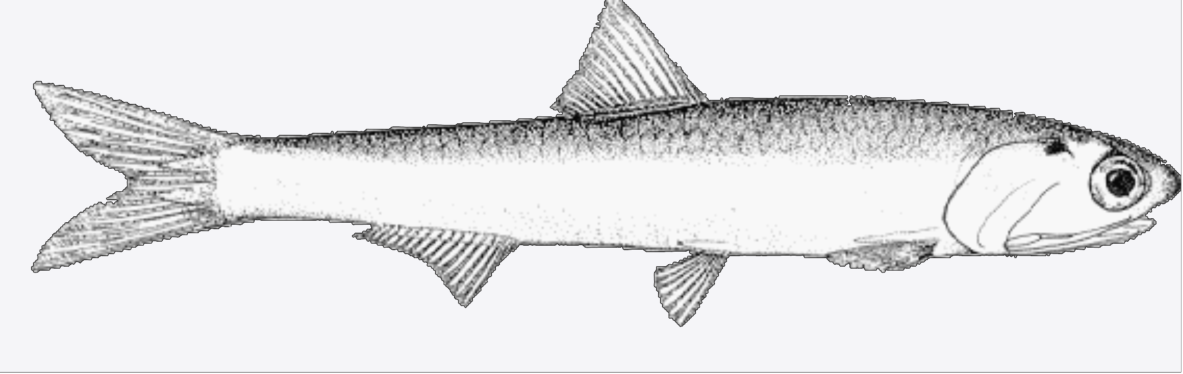
\includegraphics[scale=0.4]{figura1.pdf}  
    \caption{Anchoveta Engraulis ringens (Jenyns 1842).}
    \label{fig:figure1}
\end{figure}  

Engraulis ringens es una especie pelágica (Figura \ref{fig:figure1}) que se distribuye principalmente entre los -4$^\circ$S hasta los -42$^\circ$S, distinguiéndose tres stocks; uno que va desde el norte y centro del Perú, otro que va desde el sur del Perú al norte de Chile y el último en la zona central de Chile \citep{claramunt2012inter}. Para este estudio, el área de distribución de la anchoveta está entre el sur de Perú y norte de Chile (-16$^\circ$S $-$ -24$^\circ$S, Figura \ref{fig:figure2}) en la cual la especie constituye una unidad stock independiente del norte-centro de Perú, norte-centro y centro-sur de Chile, siendo una unidad de stock y pesquería independiente \citep{cubillos2007synchronous}.
\newline

Es importante señalar que el stock de anchoveta del sur de Perú y norte de Chile se plantea como un stock independiente del stock de anchoveta de la Región de Atacama y Coquimbo \citep{serra2012final}. \cite{canales2009parametros} plantean que la anchoveta centro-norte podría corresponder a una unidad poblacional independiente de la ubicada al norte de los -25$^\circ$S, que recluta, crece y se reproduce en el área. Los cruceros oceanográficos desarrollados en la década de 1980 muestran focos discretos de desove (huevos y larvas) de anchoveta en las bahías de Caldera y Coquimbo \citep{rojas1983estimacion}. Esto sugiere que la zona centro-norte de Chile podría representar un hábitat favorable para la anchoveta particularmente en las bahías de Caldera y Coquimbo, donde existen patrones de circulación y focos de surgencia \citep{valle2006observations} que podrían facilitar la retención y desarrollo de la anchoveta en estas bahías. \cite{sg} estudiaron la migración del stock de la anchoveta del sur de Perú y norte de Chile mostrando la ocurrencia de intensos y amplios movimientos migratorios hacia el sur de Perú en invierno y verano. Menos intensos y amplios son los movimientos migratorios de anchoveta con dirección hacia los -24$^\circ$S. Un estudio similar fue realizado por \cite{martinez1998informe} reportaron resultados similares en términos de dirección e intensidad de las migraciones. Se plantea que en la zona comprendida entre los -24$^\circ$S y -25$^\circ$S al parecer no existirían las condiciones oceanográficas para permitir un flujo continuo que permita la residencia de focos de anchoveta entre ambas zonas \todo{es una cita?}(Serra, com. pers.). Las poblaciones de Caldera y Coquimbo habrían surgido cuando en algunos años (y por razones ambientales, e.i. El Niño), la anchoveta de la zona norte expande su distribución hacia el sur de los -24$^\circ$S, colonizando las bahías de Caldera y Coquimbo donde procesos oceanográficos permiten el crecimiento y desarrollo de la anchoveta. Sin embargo, esta hipótesis no ha sido demostrada aún.

\begin{figure}[H]
    \centering
    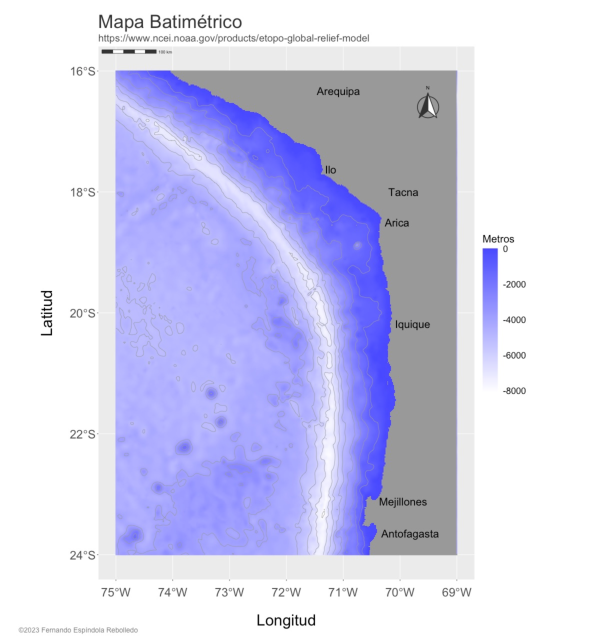
\includegraphics[scale=1.1]{figura2.pdf}  
    \caption{Área de distribución del stock de anchoveta del sur de Perú y norte de Chile, distribuido entre los -16$^\circ$S - -24$^\circ$S (FUENTE: Modelo Global de Elevación Batimétrico, ETOPO1-NOAA).}
    \label{fig:figure2}
\end{figure}  

\subsection{Fundamentos de la EEM}

% !TeX root = ../Doc_especific_mse_anchovy.tex

El IFOP es la institución de investigación encargada de brindar asesoramiento científico sobre los niveles de CBA que son consistentes con el objetivo del RMS. El modelo de evaluación que actualmente es usado con propósitos de manejo pesquero en Chile ocupa información biológica-pesquera del sur de Perú y norte de Chile. El modelo de evaluación base es estructurado a la edad con información en tallas, para lo cual se emplea una clave talla-edad dinámica en tiempo y por fuente de información, el modelo asume una escala temporal semestral con dos reclutamientos y dos desoves por año, debido al extenso período de desove (6 a 8 meses) y el rápido crecimiento observado a través de anillos diarios de otolitos \citep{cerna2016daily}. Además, incorpora las biomasas totales acústicas del sur de Perú y norte de Chile, la biomasa desovante estimada a través del método de producción diaria de huevos de Chile, los desembarques y estructuras de tamaños de las flotas comerciales para el sur de Perú y norte de Chile, y la abundancia a la talla del crucero acústico del norte de Chile. La evaluación de stock de anchoveta es actualizada dos veces al año, la primera ocurre en octubre de cada año (i) donde el stock es proyectado dos años con un supuesto en los reclutamientos futuros (4 semestres) y la segunda ocurre en marzo del año siguiente (i+1) con información actualizada completa del año anterior (i), el stock se proyecta un año incorporando una penalización en el último reclutamiento estimado por el modelo y el supuesto en los reclutamientos futuros (2 semestres).
\newline

Este procedimiento en el establecimiento de la CBA tiene un alto grado de incertidumbre. Esto se debe porque para la primera actualización, la CBA sólo depende del supuesto de reclutamiento que es ingresado en la proyección del stock. Y para la segunda actualización, la CBA depende de la forma en que es penalizado el último reclutamiento estimado por el modelo de evaluación. Esta penalización ocurre por un fuerte patrón retrospectivo en los reclutamientos que presenta el modelo de evaluación. Para la penalización del último reclutamiento se ocupan dos relaciones basadas en los reclutamientos históricos estimados por el modelo de evaluación y la biomasa de juveniles ($<$11.5 cm) que estima el crucero acústico del norte de Chile que se realiza a fines de cada año. Estas relaciones se diferencian según las condiciones ambientales (anomalías de la temperatura superficial del mar) que dominan la zona de estudio cuando se realiza el crucero acústico del norte de Chile.
\newline

El enfoque de EEM implica el desarrollo de un marco que considere el sistema de manejo pesquero en su totalidad, incluida la dinámica poblacional de los recursos y de las flotas, el esquema de recopilación de datos, el método de evaluación de poblaciones utilizado al proporcionar asesoramiento para el manejo pesquero, y cualquier regla de control de captura. El desarrollo del marco de EEM para la administración pesquera chilena es totalmente consistente con el enfoque precautorio de la FAO para la ordenación pesquera \citep{tsukamoto2008refocusing}. El desempeño de estrategias de manejo actual y candidatas para la anchoveta del norte de Chile, incluida aquella definida en el PM, no han sido aún formalmente evaluadas mediante una EEM. La regla de control que actualmente se utiliza en anchoveta del norte de Chile es modelo basada \citep{rademeyer2007tips} y se encuentra definida en el PMP (Res. Ex. 1197/2018). Sin embargo, aún no se ha evaluado formalmente el desempeño de estrategias de manejo candidatas para esta pesquería.
\newline

El diseño preliminar para el estudio de la EEM de la anchoveta del norte de Chile consistió en i) identificar los principales ejes de incertidumbre biológica para el recurso anchoveta de manera de definir un conjunto acotado de \textit{Modelos Operativos Referenciales} (MO), ii) Identificar un conjunto de \textit{Procedimientos de Manejo} (PM) pesquero y iii) identificar un conjunto adecuado de \textit{métricas de Desempeño} (MD). Estos tres principales puntos del diseño del EEM fueron acordados junto a los científicos del IFOP, administradores pesqueros de la SUBPESCA y miembros de los CCT-PP. Este documento describe las especificaciones técnicas del proceso de implementación de EEM en la pesquería de anchoveta norte y se considera en permanente revisión. Fue desarrollado en el taller presencial \textit{“Evaluación de Estrategias de Manejo para la implementación del Enfoque Precautorio en Anchoveta norte en el Contexto de la LGPA”} desarrollado en Valparaíso entre el 31 de julio al 4 de agosto del 2023.



\subsection{Introducción a openMSE}

% !TeX root = ../Doc_especific_mse_anchovy.tex

La SUBPESCA es la institución responsable de la redacción de los \textit{Términos Técnicos de Referencia} (TTR) del proyecto de determinación del estatus y posibilidades de explotación biológicamente sustentables de anchoveta y sardina española, Región de Arica y Parinacota a la Región de Antofagasta, CBA al año 2024. Este proyecto señala un nuevo objetivo (V) que requiere explícitamente la participación de los expertos internacionales que desarrollan y mantienen el software \textit{openMSE} y el uso de dicho software en la ejecución del mismo proyecto. 
\newline

openMSE es un paquete de software desarrollado en la plataforma R (R Core Team 2023), el cual es considerado como un paraguas, ya que contiene tres librerías principales para construir modelos operativos y simular la dinámica de una pesquería:

\begin{itemize}
    \item \textbf{MSEtool}: correspondiente al núcleo del paquete openMSE, el cual permite construir modelos operativos y simular la dinámica de una pesquería \citep{Hordyk2023}.
    \item \textbf{SANtool}: condicionar modelos operativos con datos y aplicar métodos de evaluación intensivos en datos \citep{Huynh2023}. 
    \item \textbf{DLMtool}: aplicar estrategias de manejo en situaciones limitadas en datos \citep{carruthers2018data}.
\end{itemize}

Los paquetes están diseñados para hacer simulaciones de la dinámica de la pesquería y el estudio del desempeño de estrategias de manejo alternativas en  un ciclo cerrado lo más simples y eficientes posible. Estos paquetes han sido aplicados en una amplia gama de pesquerías, como por ejemplo la pesquería de merluza del Pacífico Sur \citep{Hordyk2019}.
\newline

Debido a que es un conjunto de paquetes de R, los usuarios de openMSE pueden beneficiarse de todas las ventajas proporcionadas por este entorno (por ejemplo, manejo efectivo de datos, una gran colección de herramientas para el análisis de datos, funciones gráficas para el análisis y visualización de datos). Los paquetes openMSE también tienen muy buena documentación, tienen gráficos de salida bien diseñados y están hechos para que sean accesibles para todos los usuarios (no es necesario tener un alto nivel de conocimiento de R). Estas características han hecho que el software sea atractivo para los administradores pesqueros chilenos. El hecho de que el software sea de código abierto y de fácil acceso a través de la red CRAN contribuye aún más a la facilidad de comunicación y transparencia necesarias para un proceso de EEM exitoso.


\section{Componentes de una EEM}

% !TeX root = ../Doc_especific_mse_anchovy.tex

\textbf{Modelos operativos (MO)}
\newline

Los modelos operativos contienen una descripción matemática del sistema pesquero, incluida la biología de la población de peces, el patrón histórico de explotación de las flotas pesqueras y los procesos de monitoreo empleados para recopilar los datos pesqueros. Los MO también incluyen los supuestos para el proceso de monitoreo de los datos a futuro empleados en las proyecciones y cualquier error de implementación de las decisiones de manejo en las proyecciones. Un proceso de EEM incluye un conjunto de MO diferentes, cada uno de los cuales representa una hipótesis diferente sobre la posible dinámica de la pesquería. Los MO deben representar las principales fuentes de incertidumbres del sistema pesquero. De este modo la EEM permite identificar una estrategia de manejo que sea robusta a este rango de incertidumbre.
\newline

\hspace{-20pt}\textbf{Estrategia de manejo (EM)}
\newline

Las estrategias de manejo (también denominadas procedimientos de manejo) son un conjunto de reglas que convierten los datos pesqueros en recomendaciones de manejo (e.g. una captura biológicamente aceptable (CBA), una talla mínima de extracción o alguna combinación de reglas de control). El objetivo principal de la EEM es evaluar el desempeño de diferentes EM a fin de identificar un EM que sea robusto a la incertidumbre del sistema pesquero.
\newline

\hspace{-20pt}\textbf{Métricas de desempeño (MD)}
\newline

Las métricas o indicadores de desempeño se utilizan para evaluar el desempeño de los procedimientos de manejo. Las MD son indicadores cuantitativos que pueden ser calculados dentro del contexto de una EEM y de este modo se emplean para evaluar y comparar el desempeño de un conjunto de EM candidatas.


\subsection{Desarrollo de modelos operativos, modelo base.}

% !TeX root = ../Doc_especific_mse_anchovy.tex

Durante el taller presencial se identificaron un conjunto de cuatro modelos operativos (MO). Estos cuatro MOs consideró las principales fuentes de incertidumbres discutidas con mayor frecuencia en el marco de los CCT-PP, entre las que se encuentran aspectos tales como: los parámetros de crecimiento (Cerna y Plaza, 2016), la mortalidad natural y la ojiva de madurez a la talla (Hernández et al., 2023). De acuerdo con lo anterior, el MO1 corresponde al modelo base de evaluación de stock usado en el proceso actual de manejo pesquero de la anchoveta norte. El modelo base de evaluación stock es estructurado a la edad con información en tallas, para lo cual se emplea una clave talla-edad dinámica en tiempo y por fuente de información, el modelo asume una escala temporal semestral con dos reclutamientos y dos desoves por año, debido al extenso período de desove (6 a 8 meses) y el rápido crecimiento observado a través de anillos diarios de otolitos (Cerna y Plaza, 2016). Además, incorpora las biomasas totales acústicas del sur de Perú y norte de Chile, la biomasa desovante estimada a través del método de producción diaria de huevos de Chile, los desembarques y estructuras de tamaños de las flotas comerciales para el sur de Perú y norte de Chile, y la abundancia a la talla del crucero acústico del norte de Chile (Espíndola, 2023).
\newline{}

Dado el corto tiempo contemplado para la ejecución del proyecto EEM para la anchoveta norte se ha considerado esencial que el número MO’s posibles se mantenga asociado solamente con las principales fuentes de incertidumbre del MO1 que han emergido en las discusiones internas de los CCT-PP. En función de esto, se identificaron tres MO’s que se entrega en la Tabla 1.

\begin{table}[H] 
    \caption{Resumen de los modelos operativos identificados para la EEM de anchoveta norte. Las descripciones se entienden como variaciones del modelo operativo base por MO1.} 
    \label{tabla:MO}
    \begin{tabular}{cp{12cm}}
    \hline \hline
    \textbf{Identificador} & \textbf{Descripción} \\
    \hline \hline
    MO1 & Condicionado con el modelo base de evaluación de stock, incluye los parámetros de crecimiento y mortalidad natural basado en micro-incrementos diarios (Cerna y Plaza, 2016) y ojiva de madurez estimada por Martínez et al. (2009).\\
    \hline
    MO2 & Condicionado a los parámetros de crecimiento y mortalidad natural basado en macro-anillos (Serra y Canales, 2015; Plaza et al., 2012) y la ojiva de madurez del modelo operativo MO1. \\
    \hline
    MO3 & Condicionado a la ojiva de madurez presentada por Hernández et al. (2023) usando los parámetros de crecimiento y mortalidad natural del modelo operativo MO1.\\
    \hline
    MO4 & Condicionado a los parámetros de crecimiento y mortalidad natural basado en macro-anillos (Serra y Canales, 2015; Plaza et al., 2012) y la ojiva de madurez presentada por Hernández et al. (2023). \\ 
    \hline \hline
    \end{tabular}
\end{table}

A sugerencia del experto, la identificación de MO’s está en función de dos ejes de incertidumbre (parámetro de crecimiento y patrón de madurez sexual), fue organizada en una grilla de incertidumbre la que se resume en la Tabla 2: 


\begin{table}[h]
    \centering
    \caption{Grilla de incertidumbre asociada al crecimiento basado en anillos diarios y macros anillos, y la ojiva de madurez sexual usada en el modelo actual y la estimada recientemente por Hernández et. al. 2023.}
    \label{tab:tabla2}
    \begin{tabular}{|p{4.5cm}|p{3cm}|p{3cm}|}
        \hline
         & \textbf{Crecimiento actual
         (micro anillos)}
          &\textbf{Crecimiento alternativo
          (macro anillos)}
           \\
        \hline
        Ojiva de madurez actual & MO1 & MO2\\
        \hline
        Ojiva de madurez nueva & MO3 & MO4\\
        \hline
    \end{tabular}
\end{table}

Durante el taller presencial se presentaron los nuevos antecedentes sobre la ojiva de madurez sexual a la talla estimados por el Programa de Seguimiento de las Principales Pelágicas de la Zona Norte de Chile (Hernández et al. 2023) que dan cuenta de una madurez más temprana de los individuos para los años 2022, 2021 y 2020 (Figura 3). Además, se muestra la ojiva de madurez empleada en el actual modelo base de evaluación de stock (Martínez et. al., 2009). 

\begin{figure}[H]
    \centering
    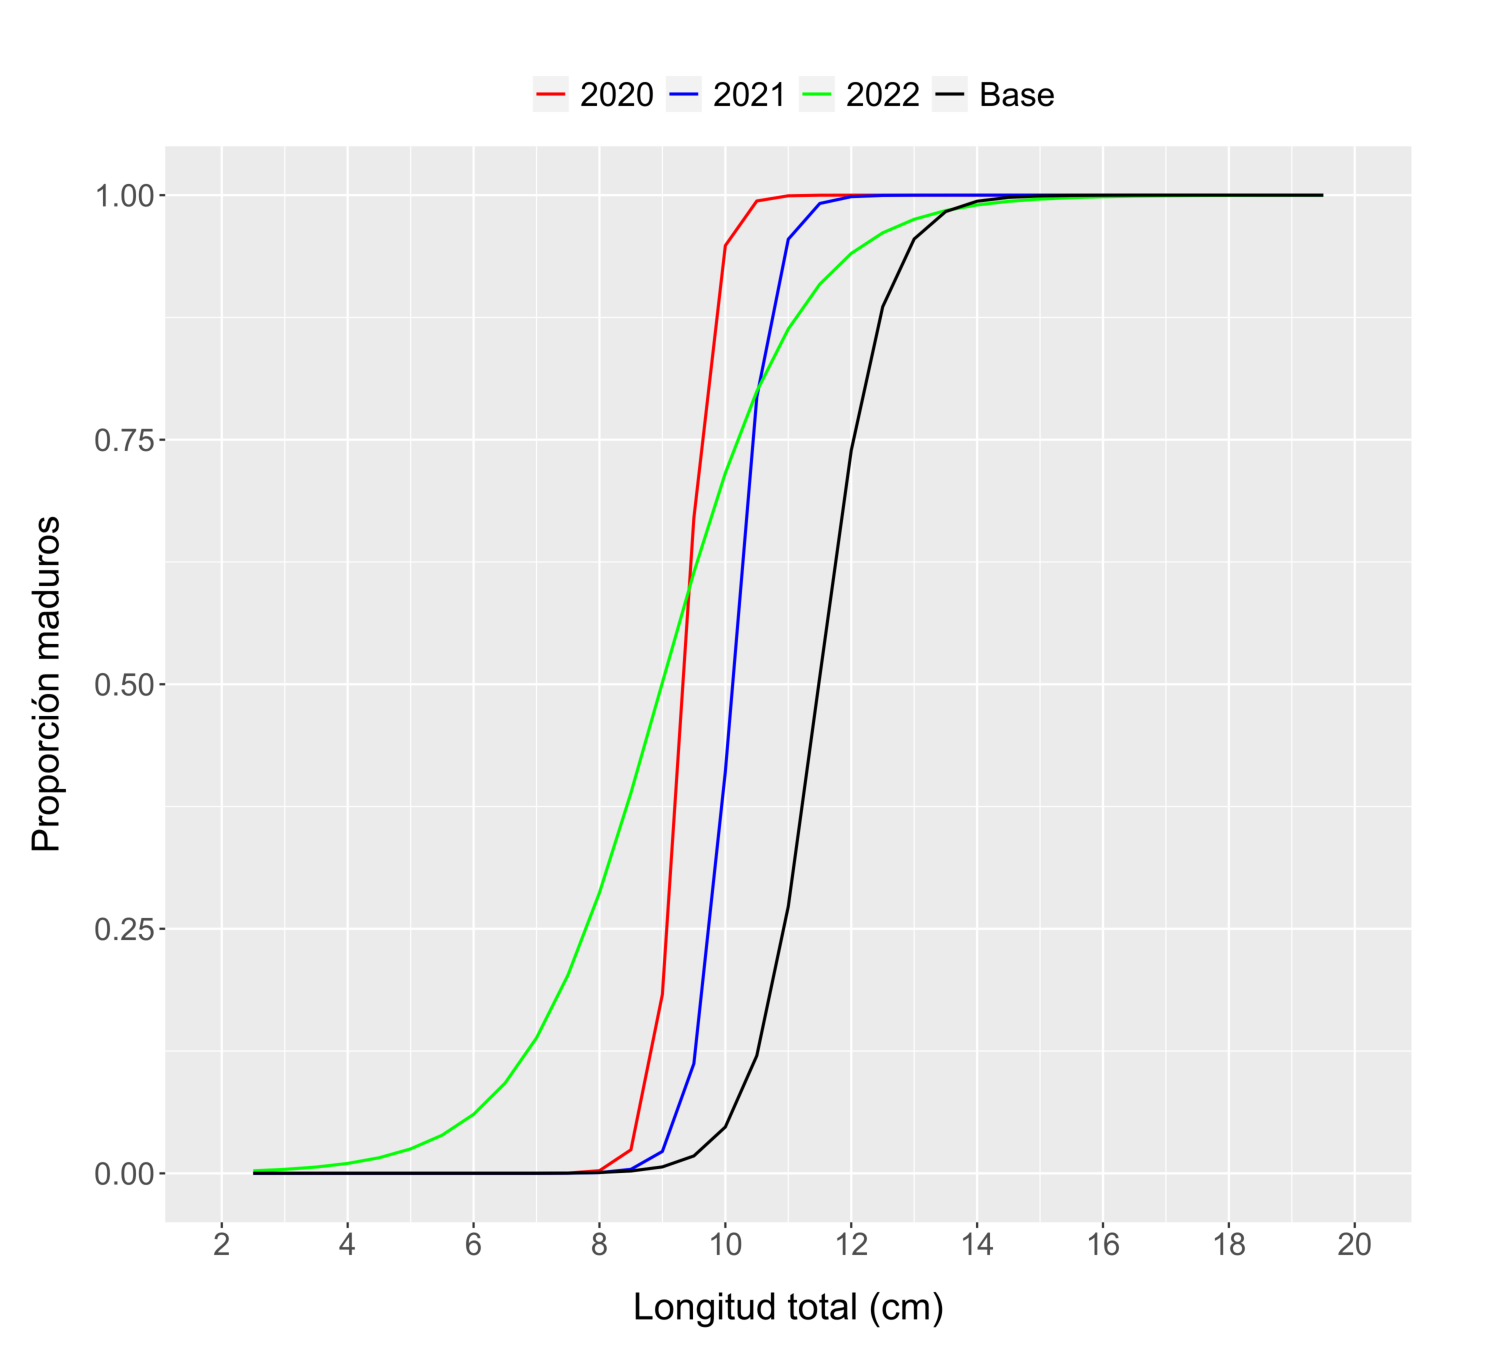
\includegraphics[scale=0.5]{figura3.pdf}
    \caption{Ojiva de madurez a la talla estimada durante los últimos los años 2020, 2021 y 2022. Además, se muestra la ojiva de madurez usada en el actual modelo base de evaluación de stock (línea negra). }
    \label{fig:figura3}
\end{figure}

\section{Supuestos de la dinámica en el MO}

% !TeX root = ../Doc_especific_mse_anchovy.tex

\subsection{Error de proceso del reclutamiento}

El error de proceso en el modelo operativo utiliza la misma desviación estándar del modelo base y considera la autocorrelación de los reclutamientos históricos tomados de las estimaciones del modelo base de evaluación de stock. Las desviaciones de los reclutamientos para el período de la proyección son generadas de una distribución log-normal, con una desviación estándar y factor de autocorrelación al primer retraso reportadas por el modelo de evaluación (Figura \ref{fig:figura4}). 
\newline

Para el modelo operativo base, la desviación estándar para las desviaciones de los logaritmos de los reclutamientos para la anchoveta fue de 0.82 con un factor de autocorrelación de -0.1868. En la Figura \ref{fig:figura5} se muestra un ejemplo de las desviaciones de los reclutamientos para nueves simulaciones.

\begin{figure}[H]
    \centering
    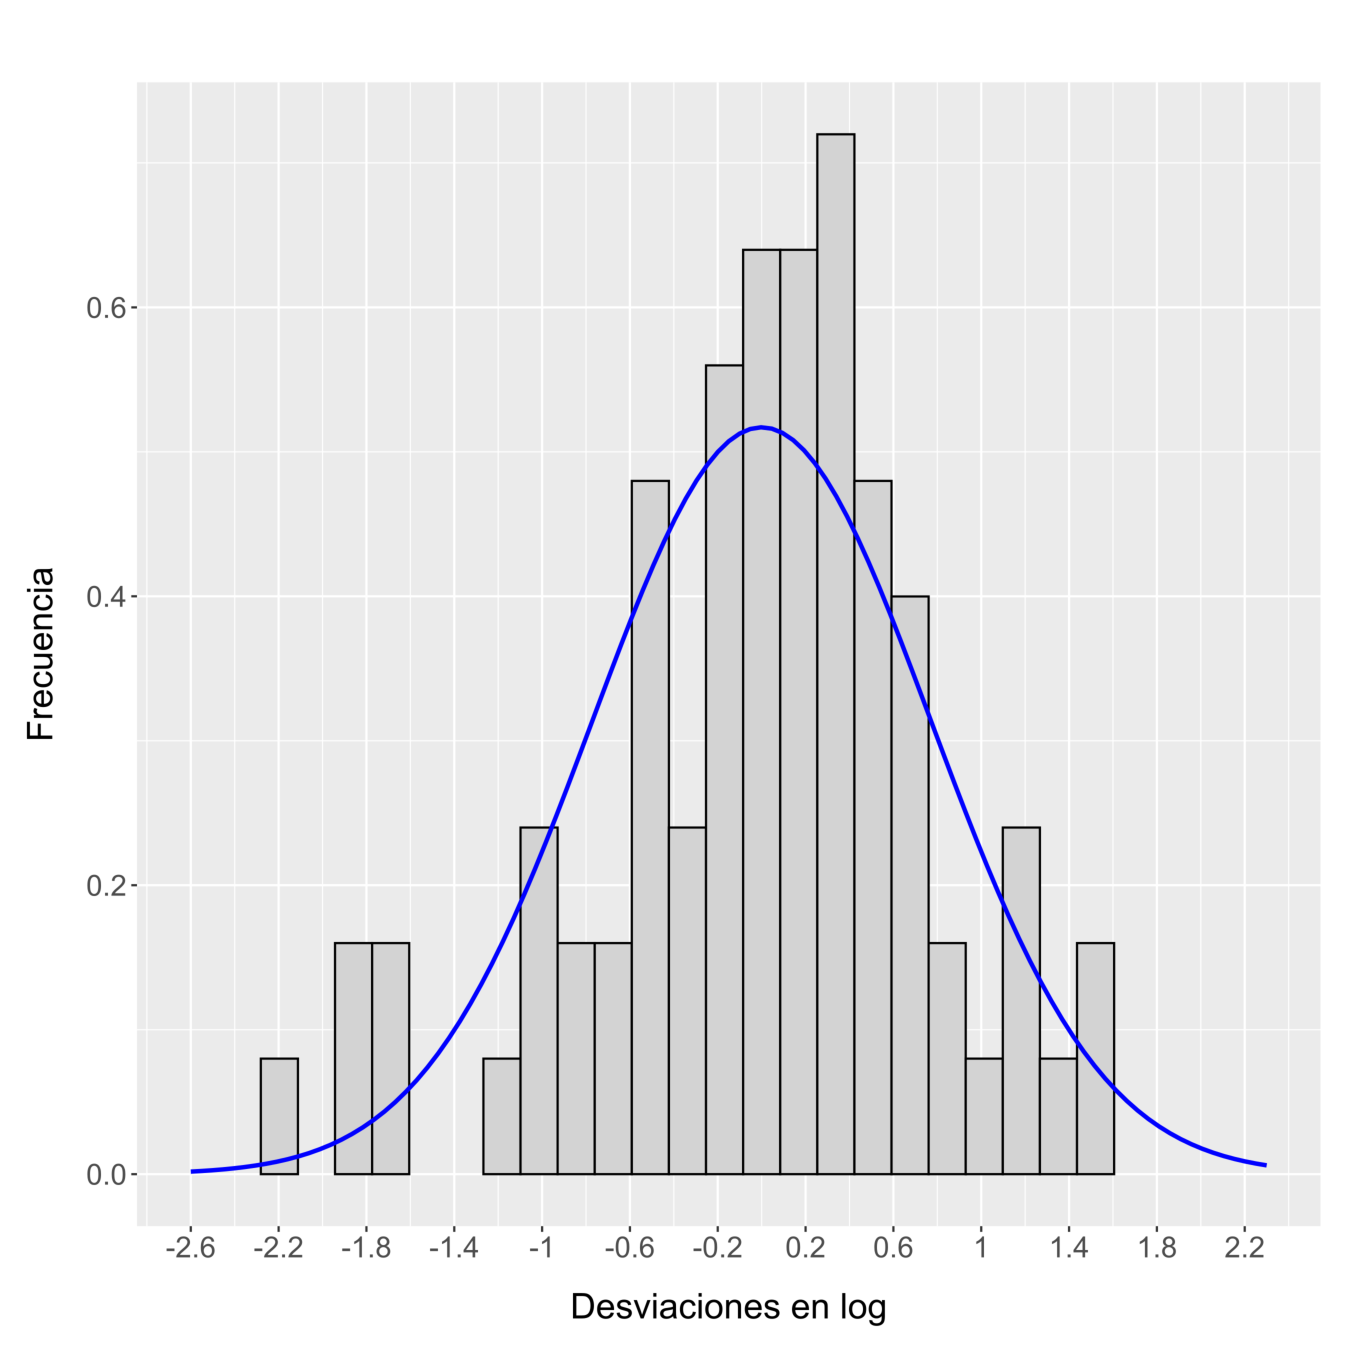
\includegraphics[scale=0.35]{figura4.pdf}
    \caption{Distribución de las desviaciones de los logarítmicos de los reclutamientos para el stock de anchoveta, la línea azul representa el ajuste de una distribución normal.}
    \label{fig:figura4}
\end{figure}

\begin{figure}[H]
    \centering
    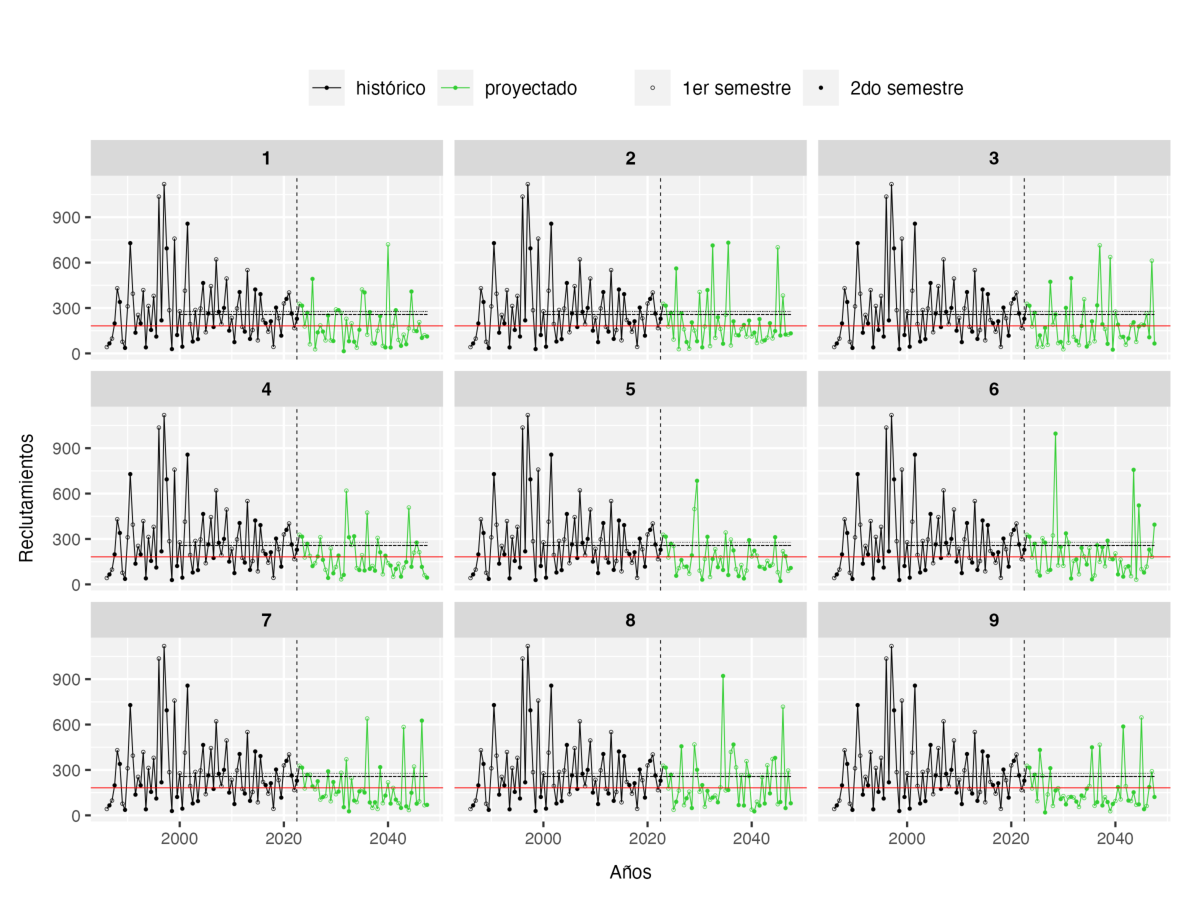
\includegraphics[scale=0.65]{value_recluta_case_om1.pdf}
    \caption{Reclutamientos proyectados para seis simulaciones del stock de anchoveta para el modelo
operativo OM1. Las líneas negras indican los reclutamientos durante el período histórico (igual para
todas las simulaciones), y las líneas verdes indican los reclutamientos en el período de la proyección, las
cuales fueron generadas a partir de una distribución de probabilidad (desviación estándar y auto-
correlacionada). La línea roja corresponde al reclutamiento medio global (R0) y las líneas discontinuas
corresponden a las estimaciones para el primer y segundo semestre del período 2000-2022.}
    \label{fig:figura5}
\end{figure}

\subsection{Parámetros de historia de vida}

Respecto a este tema, la discusión estuvo asociada a los parámetros de crecimiento y la ojiva de madurez. Los parámetros de crecimiento supuestos para el acondicionamiento de los modelos operativos se basaron en la lectura de macro anillos \citep{plaza2012}, y la lectura de micro anillos diarios \cite{cerna2016daily}. Una vez definidos los parámetros de crecimiento, se discutió sobre la ojiva de madurez presentada por \cite{Hernandez2023}. Estos resultados fueron expuestos durante el taller, donde se confirma una disminución de la talla media de madurez (L50), con una determinada variabilidad interanual (ver Figura \ref{fig:figura3} para el detalle de los escenarios alternativos). 

\subsection{Selectividad}

El patrón de selectividad para cada flota se mantuvo de acuerdo con la configuración y cambio temporal incluidos en el actual modelo de evaluación de stock para la anchoveta. 

\subsection{Error de implementación}

No hay errores de implementación explícitos en el MO. Sin embargo, de la manera que está diseñado, este error se encuentra implícito en el PM. La \textit{“hiper-regla”}, que opera en la pesquería de la anchoveta norte, determina que sin importar la CBA recomendada (en el hito 1 o 2), la CBA final siempre será la mayor de estas. De acuerdo con lo anterior, el error de implementación tiene lugar cuando la CBA adoptada es la recomendada en el primer hito.  

\subsection{Error de observación}

El error de la captura e índices de abundancia es tomado de los residuos del condicionamiento del MO. Los tamaños muestrales para la función de las muestras corresponden a los modelos de evaluación principalmente para la estructura de tamaño de la flota y crucero. Hay una diferencia entre la función de los tamaños muestrales y la función de probabilidad. El tamaño de muestra para la distribución multinomial de la composición para todas las flotas y el crucero fue fijado en 500 para representar un nivel de muestreo con alta precisión.


\section{Procedimientos de manejo (PM)}

% !TeX root = ../Doc_especific_mse_anchovy.tex

La LGPA introdujo los PMP obligatorios, estos deben especificar los objetivos, las metas y el período para reconstruir o mantener las poblaciones de peces al nivel del RMS junto con las estrategias para alcanzar los objetivos y metas establecidos. El PMP para la anchoveta norte fue aprobado el 9 de abril del 2018 (Res.Ex. N$^\circ$ 1197). Este declara una serie de objetivos operacionales asociados a estándares de manejo (indicador y punto de referencia) con los cuales se debe medir el progreso de la pesquería como consecuencia de la aplicación de medidas y/o acciones de manejo. El PMP declara llevar y mantener el stock de anchoveta a un nivel que permita asegurar la sustentabilidad biológica del recurso. Para tal efecto, el objetivo N$^\circ$1.1 es llevar y mantener el recurso al RMS, y la medida de manejo asociada a este objetivo es establecer una CBA basada en los PBR's  de la Resolución Exenta N$^\circ$291 del año 2015.
\newline

Para el caso del stock de anchoveta del norte de Chile se establecieron proxies al RMS \citep{Paya2014}, los cuales fueron ratificados por el CCT-PP. Para la BDRMS se estableció un valor igual al 50\% de la BD0, y para la FRMS se estableció aquella mortalidad por pesca que en el largo plazo produce el 55\% de la biomasa desovante por recluta (F55\%BDPR). La regla de control para este objetivo es aplicar una mortalidad por pesca constante al nivel del RMS.
\newline

Dado que el stock compartido de anchoveta es manejado en forma independiente por cada país y no existe actualmente un manejo pesquero conjunto, es necesario asumir algunas suposiciones sobre el procedimiento de manejo para la pesquería peruana. Las recomendaciones de captura para la zona sur del Perú son frecuentemente realizadas por científicos del \textit{Instituto del Mar del Perú} (IMARPE), y en su última recomendación aplicaron el modelo de producción excedentaria de \cite{jj1969generalized} re-parametrizado, estocástico y diferenciable usando información anual de la biomasa acústica estimada para la zona sur y de las capturas \citep{produce2021}. Las recomendaciones de captura hechas por el IMARPE para la zona sur del Perú son equivalentes a una tasa de explotación cercana al 0.30. Entonces, para la pesquería peruana se asume una tasa de explotación constante igual a 0.3 y la CBA que los PM producirán será asignada a la pesquería chilena, y la captura adicional peruana corresponderá al supuesto descrito anteriormente. Los procedimientos de manejo identificados, a partir de las discusiones internas del taller y entre los miembros de la SUBPESCA, sobre las prioridades de los PM para la pesquería de anchoveta norte se identificaron los siguientes:  

\begin{itemize}
    \item \textbf{Sin captura}: Se evalúa el nivel de abundancia máximo y variabilidad en el reclutamiento que puede alcanzar el stock bajo una condición sin captura (ver Figura \ref{fig:figure6}). 
    \item \textbf{Conocimiento perfecto de la abundancia del stock}: Se considera una mortalidad por pesca al 55\% de la biomasa desovante por recluta (ver Figura \ref{fig:figure6}). 
\end{itemize}


\subsection{PM actual: No se ajusta del patrón retrospectivo para la CBA.}

La evaluación de stock de anchoveta es actualizada dos veces al año. La primera actualización ocurre en octubre de cada año (i) donde el stock es proyectado cuatro semestres haciendo un supuesto acerca de los reclutamientos diferenciados por semestre y la captura igual a la CBA del año i (la captura del primer semestre ha ocurrido y la del segundo semestre es la diferencia con respecto a la CBA del año i). La segunda actualización ocurre en marzo del año siguiente (i+1) con información completa del año anterior (i), donde el stock se proyecta dos semestres nuevamente haciendo un supuesto en los reclutamientos futuros diferenciados por semestre. Las recomendaciones de la CBA son realizadas en escala anual.

\subsection{PM actual con rho de Mohn – se ajusta el patrón retrospectivo para la CBA}

El procedimiento de manejo actual tiene un alto grado de incertidumbre, ya que en la segunda actualización la CBA depende de si el último reclutamiento estimado por el modelo de evaluación es penalizado o no. Esto se debe a que el modelo de evaluación actual presenta un patrón retrospectivo positivo en los reclutamientos \citep{espinola2023}. Anticipando a que este patrón sea incorporado en la proyección, se aplica el estadístico de rho de Mohn \citep{mohn1999retrospective,hurtado2015looking,huynh2022closed} para la estimación de la CBA. Durante la proyección del stock de anchoveta, los reclutamientos
estimados al último semestre se corrigen en base al parámetro de rho de Mohn: \todo{Supongo que aquí va algo que está pendiente}
\newline

Donde es el reclutamiento ajustado, es el último reclutamiento estimado por el modelo de evaluación,
y el estadístico rho de Mohn (\todo{Aquí va la cita?}) para el reclutamiento es calculado a partir de un análisis retrospectivo, el
cual consiste en ir eliminando series de datos hasta los últimos 5 años más recientes (en pasos anuales).
Las estimaciones de un modelo consistente a lo largo del tiempo (sin patrón retrospectivo) debería
tener un . El ajuste rho se realiza en ambos pasos de tiempo del procedimiento de manejo.
\newline

El modelo de evaluación utilizado en estos dos MP es el Modelo de Acondicionamiento Rápido (RCM),
codificado en TMB y distribuido en el paquete SAMtool de R, y es una aproximación de la evaluación
actual de anchoveta codificada en ADMB. No es técnicamente factible probar la evaluación actual en
una simulación de circuito cerrado debido al tiempo de ejecución del modelo. Dado el mismo conjunto
de datos, las tendencias y la magnitud de las estimaciones históricas de la biomasa desovante son
similares entre los dos modelos (Figura \ref{fig:RCM_.ADMB}). Es importante destacar que RCM tiene el mismo
comportamiento retrospectivo (Figura \ref{fig:Retros_RCM}) que el modelo base de evaluación de stock.

\begin{figure}[H]
    \centering
    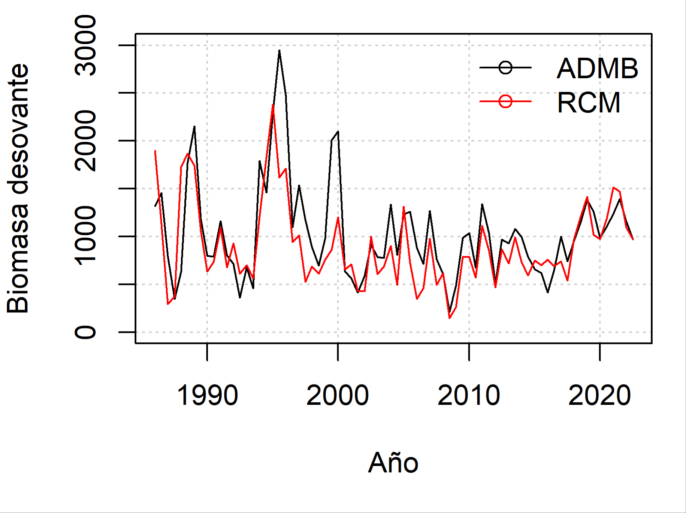
\includegraphics[scale=1.1]{RCM_.ADMB.pdf}  
    \caption{Comparación de la estimación de la biomasa desovante para el stock de anchoveta a través del
    Modelo de Acondicionamiento Rápido (RCM) y el modelo actual de evaluación en ADMB.}
    \label{fig:RCM_.ADMB}
\end{figure}  

\begin{figure}[H]
    \centering
    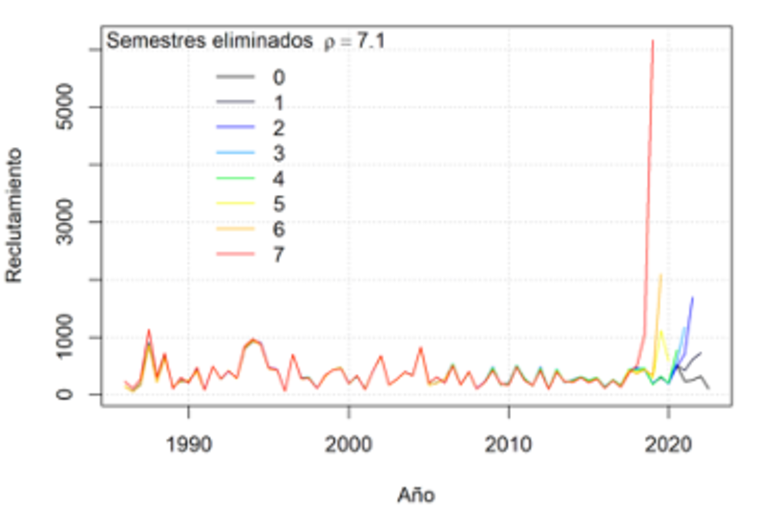
\includegraphics[scale=1.1]{Retros_RCM.pdf}  
    \caption{Patrón retrospectivo para el reclutamiento estimado para el Modelo de Acondicionamiento
    Rápido (RCM), se muestra el descuento de siete pasos de tiempo.}
    \label{fig:Retros_RCM}
\end{figure}  

\subsection{PM basado en una aproximación empírica, modelo basado simple.}

Este PM emplea la regla empírica propuesta por \cite{canales2021empirical} la que se basa en los valores de referencia en la captura y los valores de los cuantiles para la biomasa desovante estimada en el crucero de huevos. Los niveles de capturas representan los niveles históricos en las capturas semestrales de diferentes períodos.
\newline

Durante el taller presencial se acordó implementar esta regla de control usando tanto datos del crucero de huevos como del crucero acústico. El nivel de captura de referencia fue acordado para ambos casos como un valor de referencia de 285 mil toneladas, como representativo de los últimos años. Y los valores de los índices para cada caso corresponderá a los mismos criterios empleados por \cite{canales2021empirical}. 
\newline

\begin{figure}[H]
    \centering
    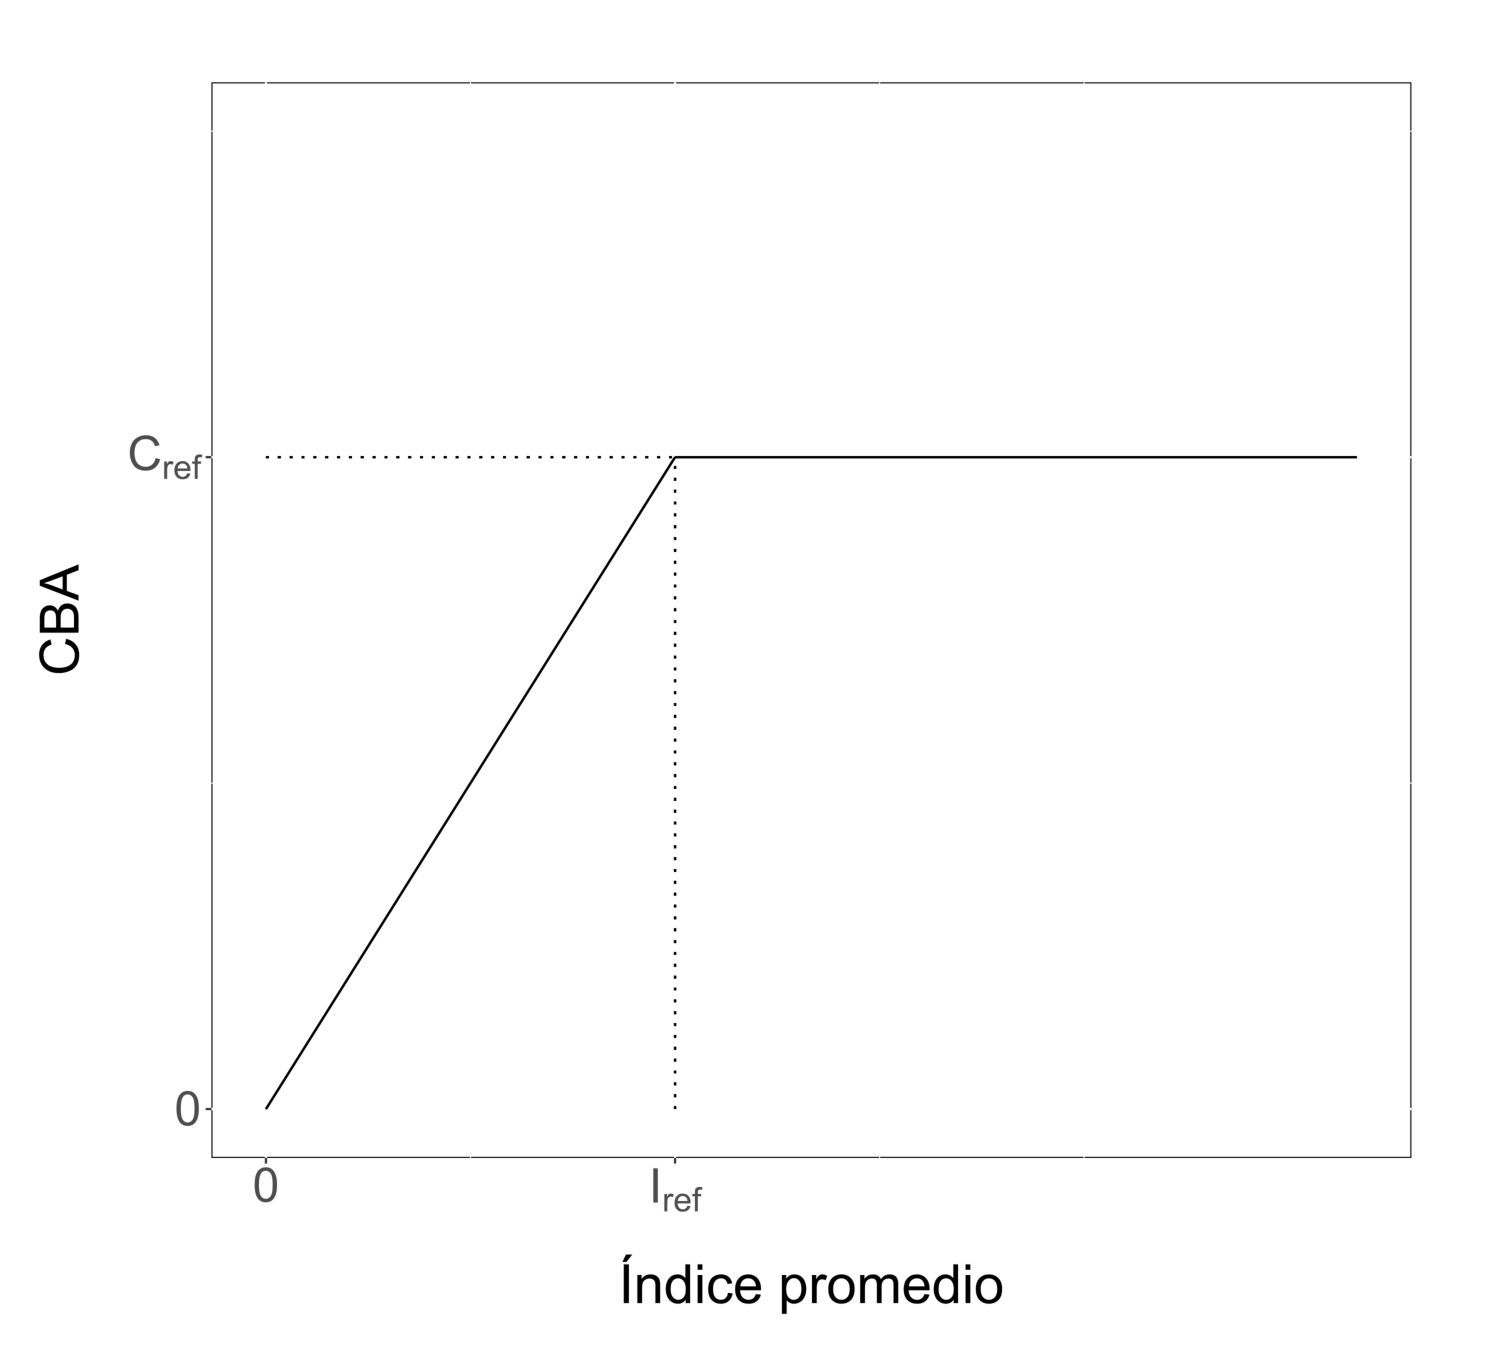
\includegraphics[scale=0.5]{cba_empirico.pdf}  
    \caption{Relación entre la captura de referencia y el índice de referencia para la regla de control de
    captura (RCC) basado en el crucero.}
    \label{fig:cba_empirico.pdf}
\end{figure} 
\todo{Ojo, esta imagen nunca se menciona en el texto}
% Con respecto a los reclutamientos se acordó: continuar con la metodología de utilizar el promedio diferenciado por semestre.

% \begin{itemize}
%     \item Para los PM establecidos se continuará con la metodología propuesta y usada habitualmente por el CCT-PP para proyectar el stock de anchoveta, promedios diferenciados por semestre \citep{espinola2023}. 
%     \item Para una futura exploración de PM se podrá explorar la inquietud señalada por la SUBPESCA, con relación a realizar un ejercicio con un sólo reclutamiento (como caso excepcional, por ejemplo, para escenarios del ENSO).
% \end{itemize}

En el Cuadro \ref{tab:tabla3} se resumen los diferentes procedimientos de manejo detallados anteriormente.

\begin{table}[H]
    \centering
    \caption{Resumen de los procedimientos de manejo en la simulación para la anchoveta norte. Las descripciones se entienden como variaciones del modelo operativo base por MO1.}
    \label{tab:tabla3}
    \begin{tabular}{|p{3.5cm}|p{10cm}|}
        \hline
        \textbf{Nombre} & \textbf{Descripción} \\
        \hline
        PM\_Actual & No se ajusta el patrón retrospectivo en el reclutamiento del último semestre.\\
        \hline
        PM\_Actual\_Rho & Se ajusta el patrón retrospectivo en el reclutamiento del último semestre.\\
        \hline
        PM\_empírico\_H & Se basa en el crucero de huevos. \\
        \hline
        PM\_empírico\_R & Se basa en el crucero acústico de reclutas. \\
        \hline
        Sin\_Captura & Procedimiento de referencia con F=0 \\
        \hline
        Manejo\_Perfecto & Procedimiento de referencia con conocimiento perfecto de la abundancia y puntos de referencia al RMS, F=55\%BDPR.\\
        \hline
    \end{tabular}
\end{table}




\section{Medidas de desempeño}

\input{./Secciones/Desempeño.tex}

\input{./Secciones/imagenes.tex}

\section{Asistentes al Workshop}

% !TeX root = ../Doc_especific_mse_anchovy.tex

\begin{table}[H]
    \centering
    \begin{tabular}{|p{3.5cm}|p{6cm}|p{4cm}|}
        \hline
        \textbf{Nombre} & \textbf{Correo} & \textbf{Institución} \\
        \hline
        Nicole Mermoud &nmermoud@subpesca.cl & SUBPESCA\\
        \hline
        Silvia Hernandez & shernandez@subpesca.cl & SUBPESCA\\
        \hline
        Víctor Espejo & vespejo@usbpesca.cl &  SUBPESCA\\
        \hline
        Camila Sagua & Scsagua@subpesca.cl & SUBPESCA\\
        \hline
        Luciano Espinoza & lespinoza@subpesca.cl & SUBPESCA\\
        \hline
        Karin Silva & ksilva@subpesca.cl & SUBPESCA\\
        \hline
        Marco Arteaga & marteaga@inpesca.cl & INPESCA\\
        \hline
        Doris Bucarey & doris.bucarey@ifop.cl & IFOP\\
        \hline
        Nicolas Adasme & nicolas.adasme@ifop.cl &  IFOP\\
        \hline
        José Zenteno & jose.zenteno@ifop.cl & IFOP\\
        \hline
        Renzo Tascheri & renzo.tascheri@ifop.cl & IFOP\\
        \hline
        Natalia Opazo & natalia.opazo@ifop.cl & IFOP\\
        \hline
        Carlos Cortes & carlos.cortes@ifop.cl &  IFOP\\
        \hline
        Alejandro Roldan & alejandro.roldan@ifop.cl & IFOP\\
        \hline
        Mauricio Ibarra & mauricio.ibarra@ifop.cl & IFOP\\
        \hline
        Fernando Espíndola & fernando.espindola@ifop.cl & IFOP\\
        \hline
    \end{tabular}
\end{table}



\bibliographystyle{apalike}
\bibliography{citas.bib}
\addcontentsline{toc}{chapter}{Bibliografía}

\end{document}
 